\section{NP-Hardness}
\begin{definition}
\emph{P} is the set of decision problems that can be solved in polynomial time. Intuitively, P is the set of problems that can be solved quickly.
\end{definition}
\begin{definition}
\emph{NP} is the set of decision problems with the following property: if the answer is \Var{Yes}, then there is a \emph{proof} of this fact that can be checked in polynomial time. Intuitively, NP is the set of decision problems where we can verify a \Var{Yes} answer quickly if we have the solution in front of us.
\end{definition}
\begin{definition}
\emph{co-NP} is essentially the opposite of NP. If the answer to a problem in co-NP is \Var{No}, then there is a proof of this fact that can be checked in polynomial time.
\end{definition}
Every decision problem in P is also in NP and also in co-NP.
\begin{definition}
A problem $\Pi$ is \emph{NP-hard} if a polynomial-time algorithm for $\Pi$ would imply a polynomial-time algorithm for every problem in NP.
\end{definition}
\begin{definition}
A problem $\Pi$ is \emph{NP-complete} if it is both NP-hard and an element of NP.
\end{definition}
\begin{theorem}[Cook-Levin Theorem]
Circuit satisfiability is NP-complete.
\end{theorem}
To prove that problem $A$ is NP-hard, reduce a known NP-hard problem to $A$.
\begin{definition}
A \emph{many-one} reduction from one language $L' \subseteq \Sigma^*$ is a function $f : \Sigma^* \rightarrow \Sigma^*$ such that $x \in L'$ iff $f(x) \in L$. A \emph{language} $L$ is NP-hard iff, for any language $L' \in NP$, there is a \emph{many-one} reduction from $L'$ to $L$ that can be computed in polynomial time.
\end{definition}
\subsection{NP-Hard Problems}
\begin{itemize}
	\item SAT
	\item 3SAT
	\item Maximum Independent Set: find the size of the largest subset of the vertices of a graph with no edges between them
	\item Clique: Compute the number of nodes in its largest complete subgraph
	\item Vertex Cover: Smallest set of vertices that touch every edge in the graph
	\item Graph Coloring: Find the smallest possible number of colors in a legal coloring such that every edge has two different colors at its endpoints
	\item Hamiltonian Cycle: find a cycle that visits each vertex in a graph exactly once
	\item Subset Sum: Given a set $X$ of positive integers and an integer $t$, determine whether $X$ has a subset whose elements sum to $t$
	\item Planar Circuit SAT: Given a boolean circuit that can be embedded in the plane so that no two wires cross, is there an input that makes the circuit output \Var{True}
	\item Not All Equal 3SAT: Given a 3CNF formula, is there an assignment of values to the variables so that every clause contains at least one \Var{True} literal \emph{and} at least one \Var{False} literal?
	\item Exact 3-Dimensional Matching: Given a set $S$ and a collection of three-element subsets of $S$, called \emph{triples}, is there a sub-collection of disjoint triples that exactly cover $S$?
	\item Partition: Given a set $S$ of $n$ integers, are there subsets $A$ and $B$ such that $A \cup B = S$, $A \cap B = \emptyset$, and $\sum_{a \in A} a = \sum_{b \in B} b$?
	\item 3Partition: Given a set $S$ of $3n$ integers, can it be partitioned into $n$ disjoint three-element subsets, such that every subset has exactly the same sum?
	\item Set Cover: Given a collection of sets $\mathscr{S} = \{ S_1, S_2, \ldots, S_m \}$, find the smallest sub-collection of $S_i$'s that contains all the elements of $\bigcup_i S_i$
	\item Hitting Set: Given a collection of sets $\mathscr{S} = \{ S_1, S_2, \ldots, S_m \}$, find the minimum number of elements of $\bigcup_i S_i$ that hit every set in $\mathscr{S}$
	\item Hamiltonian Path: Given a graph $G$, is there a path in $G$ that visits every vertex exactly once?
	\item Longest Path: Given a non-negatively weighted graph $G$ and two vertices $u$ and $v$, what is the longest simple path from $u$ to $v$ in the graph? A path is \emph{simple} if it visits each vertex at most once.
	\item Steiner Tree: Given a weighted, undirected graph $G$ with some of the vertices marked, what is the minimum-weight subtree of $G$ that contains every marked vertex?
\end{itemize}

\subsection{Hamiltonian Cycle [From Vertex Cover]}

For each vertex $u$, all the edge gadgets are connected in $H$ into a single directed path, a vertex chain. $H$ has $d-1$ additional edges for each $i$. $H$ also contains $k$ cover vertices, $1 - k$, with a directed edge to the first vertex in each vertex chain and a directed edge from the last vertex in each vertex chain.\\

Start at cover vertex 1 and traverse vertex chain for $vu_{2}$, then visit cover vertex 2 and so on and so forth before returning to 1. If $v$ is a part of the vertex cover, follow the edge from $(u_{i}, v, in)$ to $(u_{i}, v, out)$, else, detour from  $(u_{i}, v, in)$ > $(v, u_{i}, in)$ > $(v, u_{i}, out)$ > $(u_{i}, v, out)$.\\

$G$ contains a vertex cover of size $K$ if and only if $H$ contains a Hamiltonian cycle

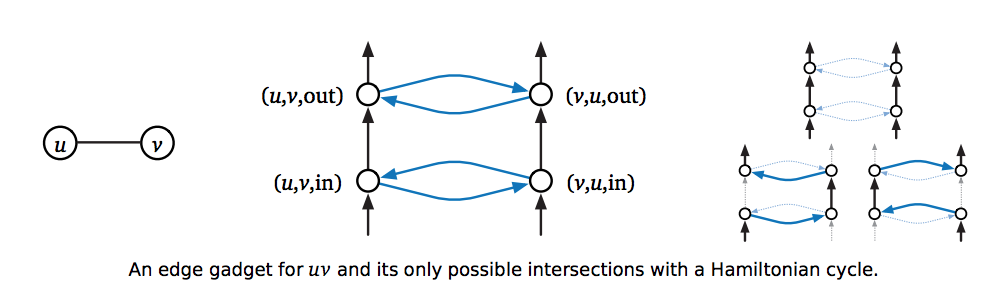
\includegraphics[width=\linewidth]{images/edgegadget.png}
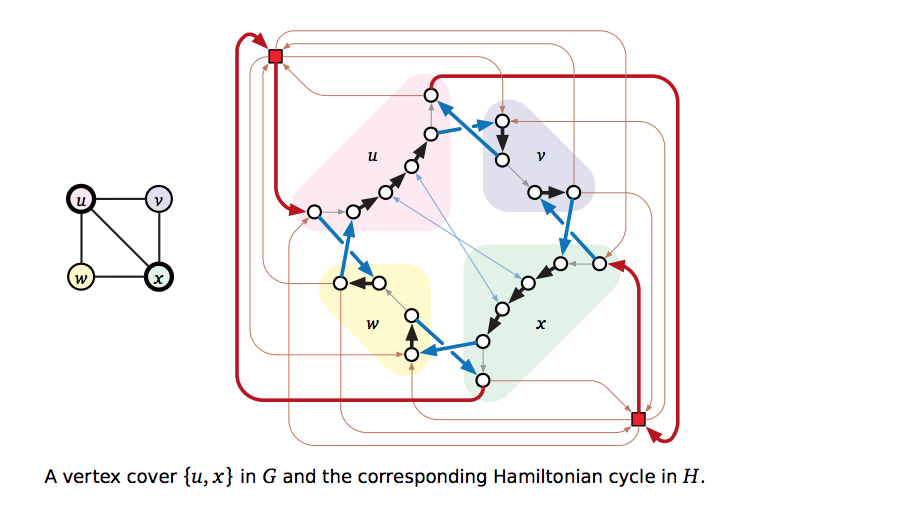
\includegraphics[width=\linewidth]{images/hamiltoniancycle.png}

\subsection{Subset Sum}

Given a graph $G$ and an integer $k$, first number edges from 0 to $m-1$; set $X$ contains the integer $b_{i} = 4^{i}$ for each edge $i$, and the integer $a_{v} = 4^{m} + \sum_{i \in \delta(v)}{4^i}$ where $\delta(v)$ is the set of edges that have $v$ as an endpoint. Finally, we set the target sum: $t = k * 4^m + \sum_{i = 0}^{m-1}{2 * 4^i}$

\subsection{Longest Increasing Subsequence [from DAG]}

Turn every number in the sequence into a vertex in a graph. Construct a special vertex $d$. For each vertex $v_1$, construct an edge to another vertex $v_2$ if (1) $v_2$ comes after $v_1$ in the sequence, and (2) $v_2$ > $v_1$. Also construct an edge to $d$.\\ 

Every path on this graph is a valid increasing subsequence. The problem of finding the LIS is now the problem of finding the longest path on this graph. Apply DAG.

\subsection{Maximum Independent Set [from 3SAT]}

Construct a graph $G$ which has one vertex for each instance of each literal in the 3SAT formula. Two vertices are connected by an edge if (1) they correspond to literals in the same clause, or (2) they correspond to a variable and its inverse. For example, the formula $(a \vee b \vee c) \wedge (b \vee \overline{c} \vee \overline{d}) \wedge (\overline{a} \vee c \vee d) \wedge (a \vee \overline{b} \vee \overline{d})$ is transformed into:

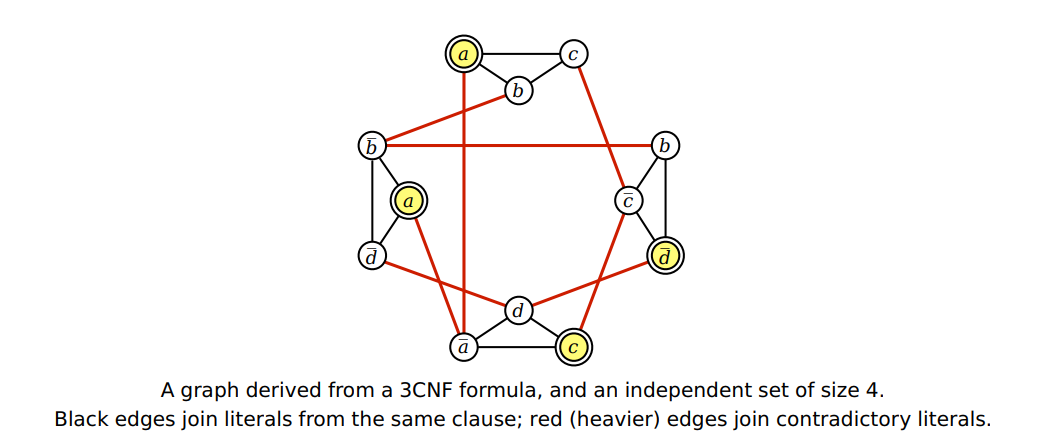
\includegraphics[width=\linewidth]{images/3CNFGraph.png}

Suppose the original formula had $k$ clauses. Then the formula is satisfiable iff the graph has an independent set of size $k$.

\subsection{Clique [from Independent Set]}
Any graph $G$ has an \emph{edge-complement} $\overline{G}$ with the same vertices, but with exactly the opposite set of edges - $(u, v)$ is an edge in $\overline{G}$ if and only if it is \emph{not} an edge in $G$. A set of vertices is independent in $G$ if and only if the same vertices define a clique in $\overline{G}$. Thus, we can compute the largest independent set in a graph by computing the largest clique in the complement of the graph.

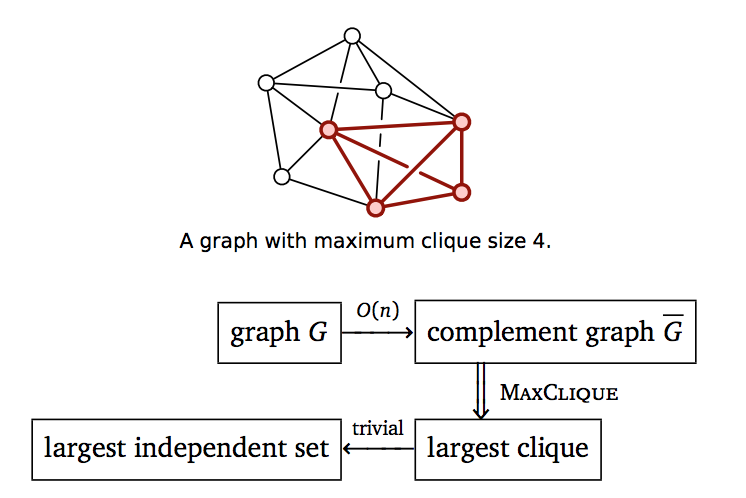
\includegraphics[width=\linewidth]{images/maxclique.png}

\subsection{3Color [from 3SAT]}

Truth gadget: $T,F$, and $X$ for true/false/other, variable gadget for variable a connecting and $\overbar{a}$ which must be opposite bools. Clause gadget joining three literal nodes to node $T$ in the truth gadget using give new unlabeled nodes and ten edges.